\section{Prototyp}
\subsection{Realisierung}
Für die Realisierung des Prototypen hat der Autor das Kennenlern-Angebot von AWS, ein einjähriges kostenloses Kontingent an Services und Produkten\cite{FreeTier2020}, gewählt. 

Nachdem der \emph{AWS Testaccount} erstellt war, mussten erste Schritte wie grundlegende Konfigurationen des Identity Access Management (IAM) gemacht und das Steuern von Spot Anfragen erlernt werden.

Weitere Schritte folgten. Die Realisierung des Prototypen wird in den folgenden Kapiteln beschrieben werden.

\begin{figure}[H]
	\centering
	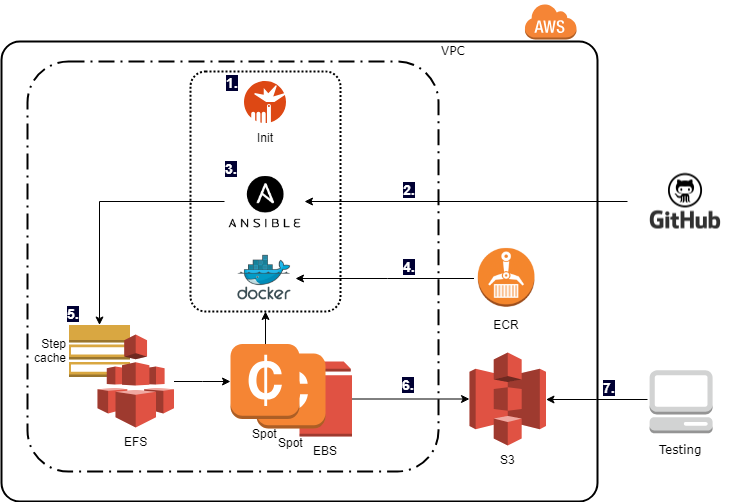
\includegraphics[width=.90\textwidth]{poc_zustand}
	\caption{Geodatenprozessierung mit SPOT Instanzen}
	\label{fig:ist_zustand}
\end{figure}

\subsubsection{Der Publikationsprozess als Code}
Aus der Abbildung \ref{fig:ist_zustand} ist ersichtlich, dass Ansible eine zentrale Rolle im Publikationsprozess einnimmt. 

\subsubsection{Handling der Interrupts}



\subsection{Testen}

\paragraph{Testen der Datenstruktur}


\paragraph{Unerwartetes Herunterfahren}


\paragraph{Real Case Szenario}
